\documentclass[a4paper, 14pt]{extarticle}%тип документа

%Русский язык
\usepackage[T2A]{fontenc} %кодировка
\usepackage[utf8]{inputenc} %кодировка исходного кода
\usepackage[english,russian]{babel} %локализация и переносы

%отступы 
\usepackage[left=2cm,right=2cm,top=2cm,bottom=3cm,bindingoffset=0cm]{geometry}

%Вставка картинок
\usepackage{graphicx}
\usepackage{wrapfig, caption}
\graphicspath{}
\DeclareGraphicsExtensions{.pdf,.png,.jpg, .jpeg}
\newcommand\ECaption[1]{%
     \captionsetup{font=footnotesize}%
     \caption{#1}}

%Таблицы
\usepackage[table,xcdraw]{xcolor}
\usepackage{booktabs}

%Графики
\usepackage{pgfplots}
\pgfplotsset{compat=1.9}

%Математика
\usepackage{amsmath, amsfonts, amssymb, amsthm, mathtools}

%Заголовок
\author{Подлесный Артём \\ группа 827}
\title{Работа 3.3.1 \\ Определение удельного заряда электрона методами магнитной фокусировки и магнетрона }

\begin{document}
\maketitle

\paragraph*{Цель работы:}исследование свободных колебаний в контуре.

\section*{Краткая теоретическая справка.}

Для колебательного контура с включенным в него сопротивлением можно написать уравнение:
\[RI+U_c=-L\frac{dI}{dt}.\]
Если продифференцировать его во времени и принять следующие обозначения: $\gamma = \frac{R}{2L}$, $\omega^2_0=\frac{1}{CL}$, то это уравнение принимает вид:
\begin{equation}
\ddot{I}+2\gamma\dot{I}+\omega^2_0I=0.
\end{equation}
В данном случае нас интересует случай, когда $\gamma\ll\omega_0$, тогда решая (1) получаем:
\begin{equation}
I= - \frac{U_0}{L\omega}e^{-\gamma t}\sin\omega t,
\end{equation}
где 
\[\omega = \sqrt{\omega^2_0 - \gamma^2}.\]
Тогда в нашем случае:
\begin{equation}
T = 2\pi\sqrt{LC},
\end{equation}
а временная зависимость напряжения:
\[U_C = U_0\exp^{-\gamma t}\cos\omega_0t.\]

При $\gamma = \omega_0$ происходит переход в апериодический режим, чему соответствует критическое сопротивление:
\begin{equation}
R_{\text{кр}} = 2\sqrt{\frac{L}{C}}.
\end{equation}

Введем добротность:
\[Q = 2\pi\frac{W}{\Delta W},\]
которая характеризует потери энергии $W$ в затухающих колебаниях, наряду с декрементом затухания:
\begin{equation}
\Theta = \frac{1}{n} \ln\dfrac{U_k}{U_{k+n}},
\end{equation}
где $U_k$ -- амплитуда k-того колебания. Если выразить добротность через параметры установки, получаем:
\begin{equation}
Q=\frac{1}{R}\sqrt{\frac{L}{C}} = \frac{\pi}{\Theta}.
\end{equation}


\section*{Экспериментальная установка}
\begin{figure}[h!]
\begin{center}
\includegraphics[width=0.7\textwidth]{ust}
\end{center}
\ECaption{Экспериментальная установка для исследования свободных колебаний.}
\end{figure}

После сборки схемы можно приступать к снятию экспериментальных данных.

\section*{Экспериментальные данные}

В работе было необходимо снять зависимости для измерения зависимости периода контура от емкости конденсатора, критическое сопротивление при котором колебательный режим переходит в апериодический, а так же исследовать затухающие колебания контура на фазовой плоскости. Далее о каждом из пунктов подробнее. 

\subsection*{Измерение периодов}

В данном случае сопротивление $R$ на магазине сопротиления выставляли равным $0$. Для расчета периода в зависимости от емкости: $T(C)$, на осциллографе, зная масштабирование оси $x$ по времени: $\Delta$, измерялась ширина, занимаемая некоторым целым числом полных периодов колебаний (что видно на осциллографе), на основании чего рассчитывался период по следующей формуле:
\begin{equation}
T = \dfrac{x\Delta}{n}.
\end{equation} 

Результаты представлены на таблице 1.

\begin{table}[h!]
\begin{center}
\begin{tabular}{|c|c|c|c|c|}
\hline
\rowcolor[HTML]{9698ED} 
$C$, мкФ   & $\Delta$, мс/см & $n$ & $x$, см   & $T$, мс    \\ \hline
0.02 & 0.2    & 3 & 5   & 0.33 \\ \hline
\rowcolor[HTML]{9698ED} 
0.11 & 0.5    & 3 & 5.6 & 0.93 \\ \hline
0.2  & 0.5    & 3 & 6.4 & 1.07 \\ \hline
\rowcolor[HTML]{9698ED} 
0.29 & 0.5    & 3 & 7.8 & 1.30 \\ \hline
0.38 & 1      & 5 & 7.4 & 1.48 \\ \hline
\rowcolor[HTML]{9698ED} 
0.47 & 1      & 4 & 6.6 & 1.65 \\ \hline
0.56 & 1      & 4 & 7.2 & 1.80 \\ \hline
\rowcolor[HTML]{9698ED} 
0.65 & 1      & 4 & 7.8 & 1.95 \\ \hline
0.74 & 1      & 3 & 6.2 & 2.07 \\ \hline
\rowcolor[HTML]{9698ED} 
0.83 & 1      & 3 & 6.6 & 2.20 \\ \hline
0.9  & 1      & 3 & 6.8 & 2.27 \\ \hline
\end{tabular}
\ECaption{Зависимость периода электрических колебаний $T$ от емкости конденсатора $C$ в контуре.}
\end{center}
\end{table}

\subsection*{Критическое сопротивление и декремент затухания}

Приняв $L=200$ мГн, можно найти емкость конденсатора, которая нужна для того, чтобы частота собственных колебаний была равна $\nu_0=5$ кГц по следущей формуле:
\[C = (4\pi^2\nu^2_0L)^{-1} = 0.005 \text{ мкФ},\]
откуда по формуле (4):
\begin{equation}
R_{\text{кр}} = 2\sqrt{\frac{L}{C}} \approx 13 \text{ кОм}.
\end{equation}

Плавно изменяя сопротивление, можно поймать момент, когда колебания становятся апериодичными. Исходя из этого "подбора" получаем такое сопротивление:
\[R_{\text{кр}} = 9500\text{ Ом}.\] 
Оно сильно отличается, однако это только потому, что индуктивность не совпадает с реальным значением.

Найдем зависимость декремента затухания в зависимости от сопротивления магазина, в области $0.1R_{\text{кр}}\div0.3R_{\text{кр}}$, при известной емкости. Декремент затухания считается по формуле (5). Эта зависимость представлена на таблице 2.

\begin{table}[h!]
\begin{center}
\begin{tabular}{|c|c|c|c|c|c|}
\hline
\rowcolor[HTML]{9698ED} 
$R/R_{\text{кр}}$ & $R$, Ом & $n$ & $U_k$, см & $U_{k+n}$, см & $\Theta$ \\ \hline
0.1              & 950  & 2   & 5.6   & 1.6       & 0.626    \\ \hline
\rowcolor[HTML]{9698ED} 
0.13             & 1235 & 2   & 4.7   & 1         & 0.774    \\ \hline
0.16             & 1520 & 2   & 4     & 0.6       & 0.949    \\ \hline
\rowcolor[HTML]{9698ED} 
0.19             & 1805 & 2   & 3.3   & 0.4       & 1.055    \\ \hline
0.22             & 2090 & 2   & 6.8   & 0.5       & 1.305    \\ \hline
\rowcolor[HTML]{9698ED} 
0.25             & 2375 & 1   & 5.7   & 1.2       & 1.558    \\ \hline
0.28             & 2660 & 1   & 4.8   & 0.8       & 1.792    \\ \hline
\rowcolor[HTML]{9698ED} 
0.3              & 2850 & 1   & 4.2   & 0.6       & 1.946    \\ \hline
\end{tabular}
\ECaption{Зависимость декремента затухания колебаний $\Theta$ от сопротивления $R$, установленного на магазине сопротивлений.}
\end{center}
\end{table}

\subsection*{Колебания на фазовой плоскости}
С помощью осциллографа были проведены наблюдения колебаний на фазовой плоскости, для 2 значений $R$ в близи нижней и высшей границ измерения декремента затухания цепи. Эти картины представлены на рис. 2.

%\begin{figure}[h!]
%\begin{center}
%\includegraphics[width=1\textwidth]{foto}
%\end{center}
%\ECaption{Картины колебаний на фазовой плоскости для 4 значений $R$ в контуре, слева на право: 0.1, 0.12, 0.28, 0.3 от $R_{\text{кр}}$. Из-за искажений при печати они могут выглядеть нечетко, однако в цифровом варианте на них четко видны линии, по которым можно посчитать необходимые значения.}
%\end{figure}

 Отсюда отношение амплитуд можно определить по отношению расстояний пересчений витков с осями,что соответствует амплитудам колебаний, разделенными целым числом периодов. Благодаря цифровой картине, можно существенно повысить точность измерения этих аплитуд, тк можно игнорировать цену деления осциллографа. 

Оммическое сопротивление катушки и её индуктивность измерялись с помощью LСR-измерителя на переменном токе. Данные представлены на таблице 3.

\begin{table}[h!]
\begin{center}
\begin{tabular}{|c|c|c|c|}
\hline
\rowcolor[HTML]{9698ED} 
$f$, Гц     & 50    & 1000  & 5000  \\ \hline
$R_{L}$, Ом & 10.2  & 12.6  & 20.1  \\ \hline
\rowcolor[HTML]{9698ED} 
$L$, мГн     & 150.2 & 144.4 & 145.4 \\ \hline
\end{tabular}
\ECaption{Результаты измерений LCR. Как видно, при изменении частоты, меняется и оммическое сопротивление. Это связано с тем, что при измерении в контуре возникают вынужденные колебания, и импеданс колебаний зависит от частоты генератора.}
\end{center}
\end{table}

\section*{Обработка экспериментальных данных.}

\subsection*{Соответствие теоретических и экспериментальных периодов колебаний контура}

Так как частота контура лежит в диапазоне $1000\div5000$ Гц, то возьмем следующее значение для индуктивности катушки: $L = 145$ мГн. Тогда по формуле получаем зависимость $T_{\text{эксп}}(T_{\text{теор}})$, представленная на рис. 3.

\begin{figure}[h!]
\begin{center}
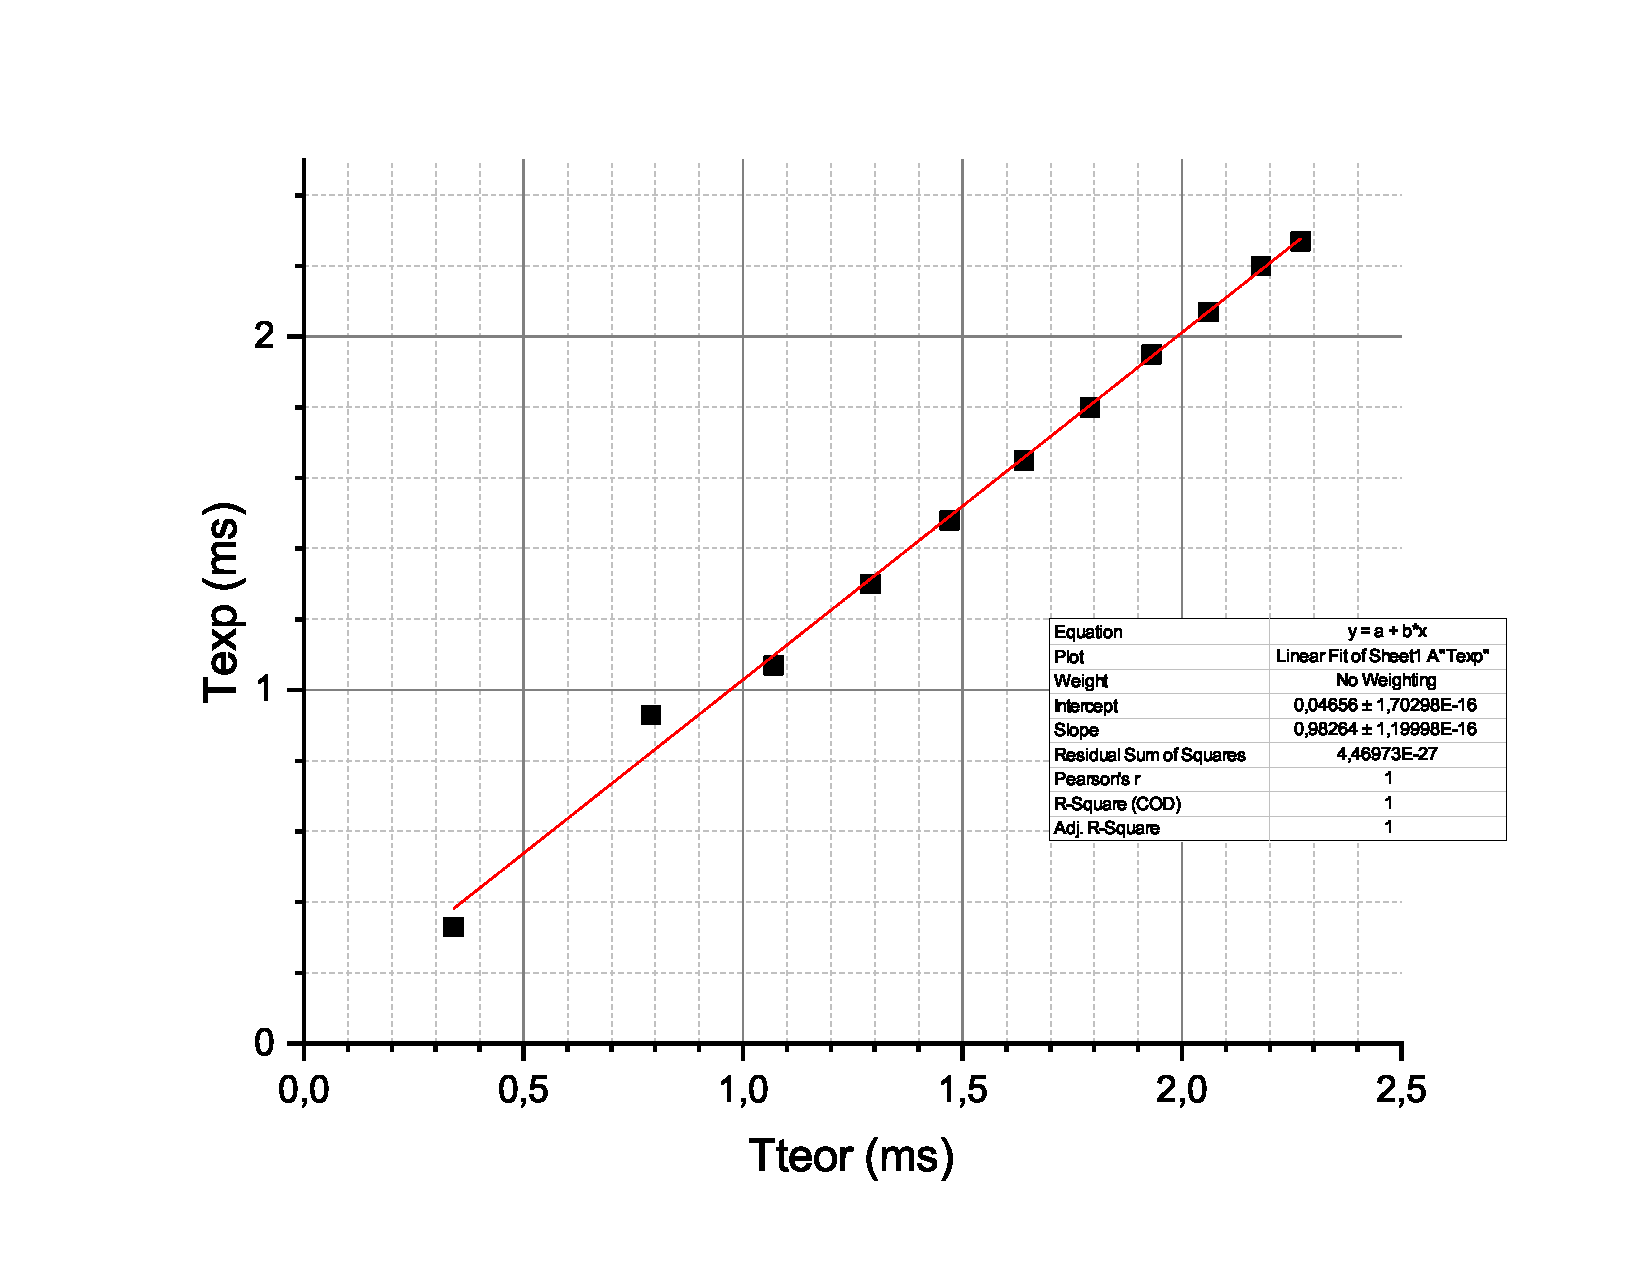
\includegraphics[width=0.8\textwidth]{TT}
\end{center}
\ECaption{График зависимости $T_{\text{эксп}}(T_{\text{теор}})$. На графике видно, что только 1 точка не ложится на прямую, имеющую коэффициент наклона крайне близкий к еденице. Эта точка скорее всего является результатом неправильной интерпретации картинки на осциллографе. }
\end{figure}

Этот график позволяет утверждать, что осциллограф крайне точно передает картину колебаний, легкое несоответствие результатов вызвано лишь несовершенством установки. 

\subsection*{Расчет критического сопротивления через декремент затухания}

Формула для расчета критического сопротивления:
\begin{equation}
R_{\text{кр}} = 2\pi\sqrt{\alpha},
\end{equation}
где $\alpha$ -- коэффициент наклона графика следующей зависимости:\\ $1/\Theta^2 = f(1/R_{\text{конт}})$, где $R_{\text{конт}} = R+R_L$.  Этот график показан на рис. 4. Для данной емкости частота соответствует 5900 Гц, поэтому $R_L = 20\pm2$ Ом, $L = 145.4\pm9.0$ мГн. 

\begin{figure}[h!]
\begin{center}
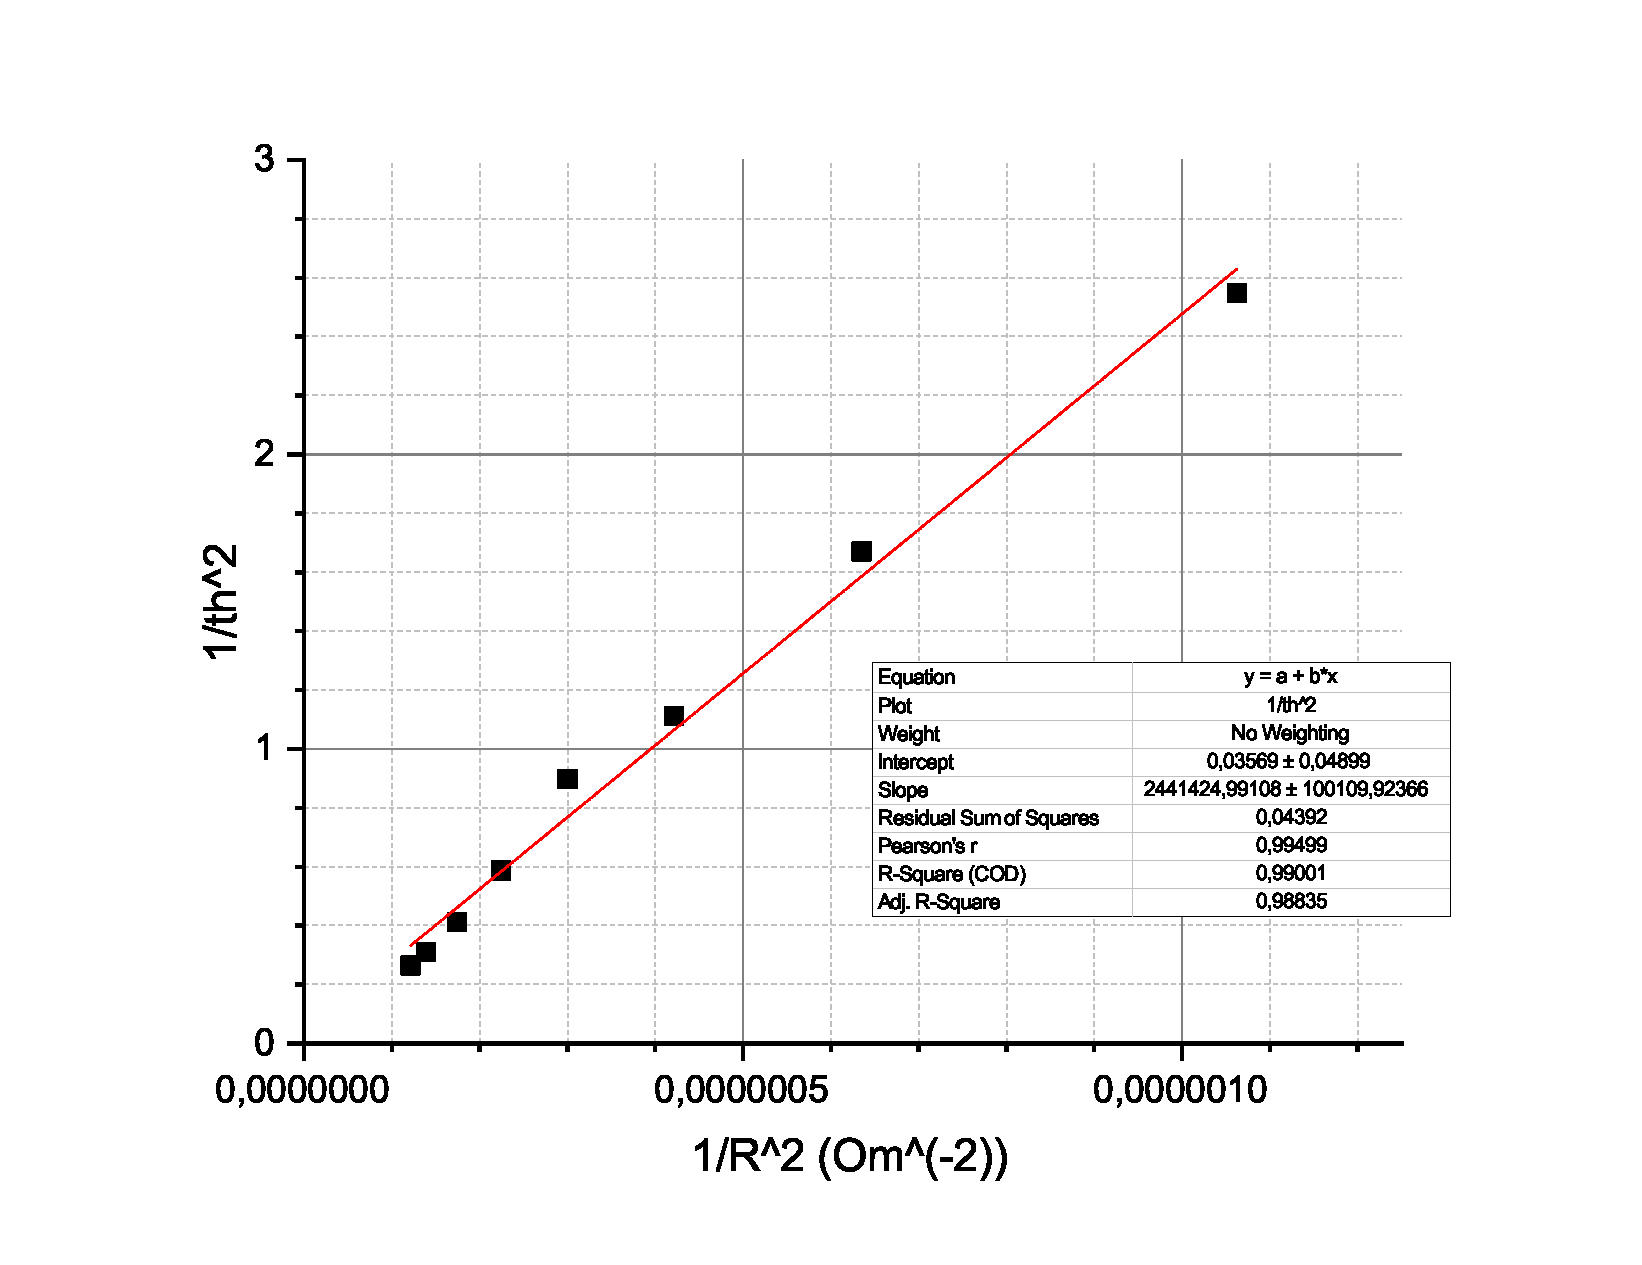
\includegraphics[width=0.8\textwidth]{THR}
\end{center}
\ECaption{График зависимости $1/\Theta^2 = f(1/R_{\text{конт}})$. Точки на графике не слишком хорошо ложатся на прямую, и, скорее всего, это из-за того, что значение $R_L$ было измерено при другой частоте, чем частота контура в этом эксперименте. }
\end{figure}

Получаем значение коэффициента наклона этого графика:
\[\alpha = (2.44\pm0.10)\times10^6 \text{ Ом}^2,\]
откуда:
\[R_{\text{кр}} = 9.8\pm0.4 \text{ kОм}.\]
Как видно, этот результат согласуется с определенным качественно по картине колебаний на осциллографе. Теоретически посчитаем критическое сопротивление по формуле (2):
\[R_{\text{кр}_\text{теор}} = 10.8\pm0.7\text{ kОм}.\]
С учетом погрешности результаты согласуются, хотя точность оставляет желать лучшего.

\subsection*{Расчет добротности контура}

Расчет добротности проводился для максимального и минимального сопротивлений резистора: 0.1 и 0.3 от критического сопротивления. По формуле (6) можем рассчитать добротности по данным установки и по декременту затухания. Они будут представлены в секции "Результаты". Так же использовался метод расчета добротности по спиралям на фазовой плоскости. Для этого с помощью k-радиусов спирали отсчитывались декремент затухания, а из него по формуле (6) - добротность.

\subsection*{Результаты}

Для того, чтобы было удобно сравнить результаты, они оформлены в виде таблицы 4.



\section*{Вывод}

Были исследованы свободные колебания в контуре, и разными методами получены ответы на поставленные вопросы. Теперь можно сравнить их и дать характеристику разным методам. Для измерения $R_{\text{кр}}$ лучше использовать метод графика с использованием декремента затухаания. Так будут получены более точные результаты. Проблемы расчета с помощью формулы (4) в том, что $L$ и $R$ зависят от частоты контура, что создает дополнительную погрешность, так как в работе индуктивность и сопротивление катушки измеряны при другой частоте, чем возникает в контуре с используемой емкостью. Подбором можно получить лишь качественную оценку критического сопротивления, однако по близости к нему можно определить достоверность остальных результатов, так как при этом сопротивлении ясно виден перееход колебаний в апериодичный режим. 

Расчет добротности через параметры установки имеет ту же проблему, но с учетом погрешности согласуются со значениями, полученными методом спирали - самым точным методом. Его точность выше, потому что можно точнее определить деркемент затухания.






\end{document}